%\vspace{1em}
%La implementación comentada del algoritmo de Kruskal parece eficiente cuando se trata de grafos ralos pero resulta menos que satisfactoria cuando se trata de estructuras más densas. En particular en este problema, se están ordenando $O(n^2)$ aristas a pesar de que solo se observan $n-1$ de ellas como máximo.

%Afortunadamente contamos con la siguiente especificación: https://fedelebron.com/a-dense-version-of-kruskals-algorithm, que detalla cómo esbozar un algoritmo no sólo más eficiente sino que asintóticamente superior, con complejidad temporal de $O(n^2)$ en vez de $O(n^2logn)$

Para revisar de manera empírica la diferencia en eficiencia entre una implementación de \textsc{modems} sobre el algoritmo de \textit{Kruskal} para grafos \textit{densos}\footnote{Para este algoritmo, nos basamos en la implementación propuesta por Federico Lebron en su \href{https://fedelebron.com/a-dense-version-of-kruskals-algorithm}{\color{blue} blog}.} y una implementación sobre el mismo algoritmo para grafos \textit{ralos}\footnote{Ver nota al pie \ref{foot_1}. Sección 23.2: \textit{The algorithms of Kruskal and Prim}.}, procedimos a implementar\footnote{Los experimentos, algoritmos y archivos resultantes se pueden encontrar en \textit{./ej-3/experimentacion}.} ambas versiones en C$++$ y realizamos una serie de evaluaciones respecto al tiempo de ejecución en función del tamaño de la entrada, para muestras aleatorias de tamaño $N = 5000k$ para cada $k$ natural en el rango $1 \leq k \leq 10$. 

Realizamos cada evaluación diez veces para reducir la variación de los resultados y tomamos el promedio aritmético. 
A su vez, controlamos los parámetros de la función de la siguiente forma. Elegimos \mbox{$W = N/4$}, $R = 1$ y $W = V = 5$, y definimos la posición de cada oficina $o_i = (x_i,\ y_i)$, para todo $0 \leq i \leq 5000k$, como la tupla $(z,\ z+1)$ para algún $0 \leq z \leq 5000k$. 

%\vspace{0.5em}
\begin{figure}[!htbp]
    \subfloat{\includegraphics[scale=0.40, clip]{./files/src/.media/comparacion_asintótica.png}}
    %\hfill
    $\ \ \ \ $
    \subfloat{\includegraphics[scale=0.4, clip]{./files/src/.media/comparacion_asintótica_diff.png}}

    \caption{Izquierda: tiempo de ejecución de \textsc{modems} en función del tamaño de entrada $N$ para el algoritmo \textit{cuadrático} ---en base a \textit{Kruskal} para grafos densos--- y el \textit{supercuadrático} ---en base a \textit{Kruskal} para grafos ralos---. Derecha: la diferencia absoluta entre ambas mediciones descripta por una regresión cuadrática.}
    \label{grafico_1}
\end{figure}

Notar que ninguna de estas decisiones afecta la complejidad asintótica del algoritmo. Sin embargo, un analisis en mayor profundidad debería, también, evaluar el comportamiento de ambos algoritmos en función de estos parámetros.

La Figura \ref{grafico_1} expone los resultados. Podemos notar que hay una clara diferencia de velocidad a favor del algoritmo cuadrático, incluso en las entradas de menor tamaño. La regresión se realizó con cuadrados mínimos y obtuvo un error, relativamente chico, de $\approx 21.17$. Esto parece indicar que la relación entre la complejidad de ambos algoritmos es superlineal. %Si bien es útil, cabe aclarar que esta observación está lejos de ser conclusiva en términos estrictamente empíricos. %Podemos concluir entonces que resulta más eficiente para este problema

\subsection{Heurísticas para la implementación de disjoint set}

Del mismo modo que realizamos la comparación anterior, también vale la pena evaluar la diferencia de tiempos que se pueden obtener al utilizar la estructura de \textit{disjoint set}, sin alguna de sus optimizaciones, en el algoritmo supercuadrático. En este caso obviaremos las heurísticas de \textit{union by rank} y \textit{path compression}. 

Esta segunda versión del algoritmo utiliza la implementación de \textit{Kruskal} para grafos \textit{ralos} sobre una estructura ingénua de \textit{disjoint set}: a la hora de unir dos conjuntos, recorremos uno ---elemento por elemento---, y lo agregamos al otro. Se puede demostrar, en base al análisis que realiza [Cormen]\footnote{Ver nota al pie \ref{foot_1}. Sección 21: \textit{Data Structures for Disjoint Sets}.}, que el algoritmo resultante tiene una complejidad temporal en $\Theta(m\log n + n^2)$, correspondiente al costo de ordenar las aristas del grafo de entrada y el costo amortizado de realizar $\Theta(n)$ operaciones sobre esta estructura de datos. En comparación, la versión utilizada en la sección anterior tiene una complejidad temporal en $\Theta(m\log n + m\alpha(n))$, donde $\alpha$ es la función inversa de \textit{Ackermann}. Si bien esto no modifica la complejidad del algoritmo, ciertamente resulta posible que afecte su tiempo de ejecución.

En forma análoga a la experimentación anterior, hicimos una prueba empírica con las dos versiones de esta implementación. La Figura \ref{fig2} muestra los resultados.

\begin{figure}[!htbp]
    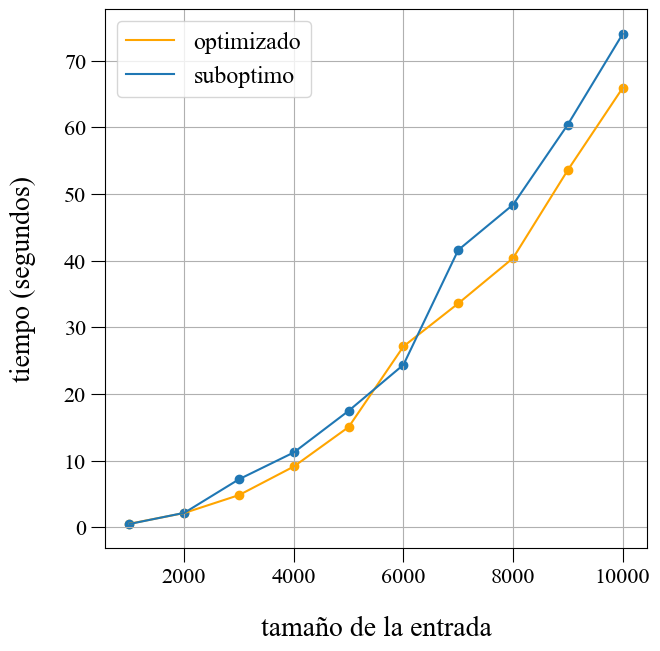
\includegraphics[scale=0.4, clip]{./files/src/.media/comparacion_DSU.png}
    \caption{Tiempo de ejecución del \textsc{modems} en función del tamaño de entrada $n$ para el algoritmo supercuadrático \textit{optimizado} ---con las heurísticas--- y \textit{subóptimo} ---o, ingénuo---.}\label{fig2}
\end{figure}

Notamos que, en las entradas más grandes, la versión sin optimizar parece funcionar mejor. Esto tiene sentido, ya que $\Theta(n^2) < \Theta(m\alpha(n))$ si el grafo de entrada es \textit{denso}. 
